\documentclass[11pt,letterpaper]{article}
\usepackage[lmargin=1in,rmargin=1in,tmargin=1in,bmargin=1in]{geometry}
\usepackage{../style/homework}
\usepackage{../style/commands}
\setbool{quotetype}{true} % True: Side; False: Under
\setbool{hideans}{false} % Student: True; Instructor: False

% -------------------
% Content
% -------------------
\begin{document}

\homework{8: Due 03/29}{You only live once, but if you do it right, once is enough.}{Mae West}

% Problem 1
\problem{10} Give a rough sketch of the quadratic function $y= 8 - (x + 7/2)^2$. Your sketch should include the vertex and axis of symmetry. 
	\[
	\fbox{
	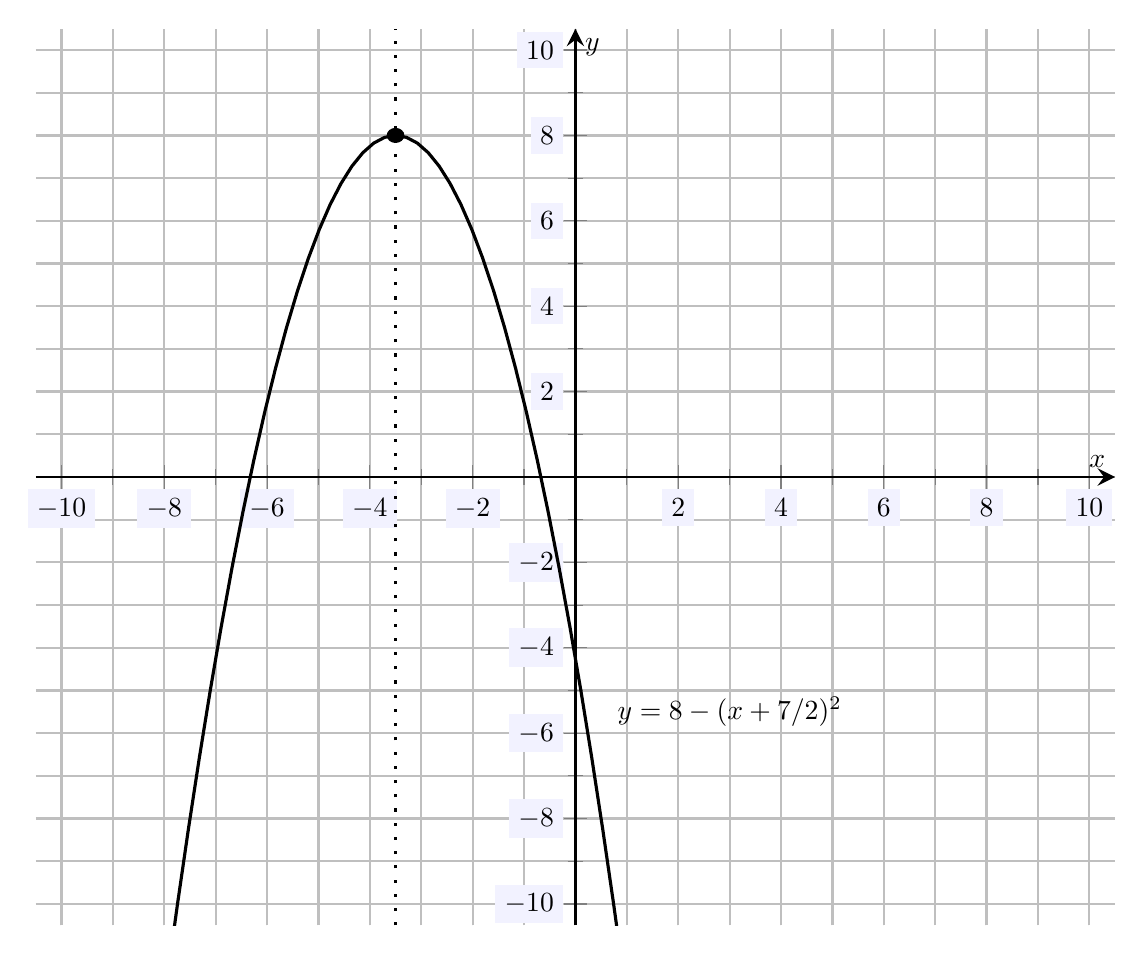
\begin{tikzpicture}[scale=2,every node/.style={scale=0.5}]
	\begin{axis}[
	grid=both,
	axis lines=middle,
	ticklabel style={fill=blue!5!white},
	xmin= -10.5, xmax=10.5,
	ymin= -10.5, ymax=10.5,
	xtick={-10,-8,-6,-4,-2,0,2,4,6,8,10},
	ytick={-10,-8,-6,-4,-2,0,2,4,6,8,10},
	minor tick = {-10,-9,...,10},
	xlabel=\(x\),ylabel=\(y\),
	]
	\node at (3,-5.5) {$y= 8 - (x + 7/2)^2$};
	\draw[fill=black] (-7/2,8) circle (0.15);
	\draw[line width=0.02cm,dotted] (-7/2,-10.5) -- (-7/2,10.5);
	\addplot[line width= 0.02cm,samples=100,domain= -10.5:10.5] ({x},{8 - (x + 7/2)^2}); 
	\end{axis}
	\end{tikzpicture}
	}
	\] \pspace

\sol We place the quadratic function in vertex form, i.e. $y= (x - p)^2 + q$. We have\dots
	\[
	y= 8 - (x + 7/2)^2= -(x + 7/2)^2 + 8= -\left(x - \dfrac{-7}{2} \right)^2 + 8
	\]
Therefore, we have vertex $(-7/2, 8)$. The axis of symmetry is then $x= -\frac{7}{2}$. Because $a= -1 < 0$, the parabola opens downwards. This gives us the sketch above. 




\newpage



% Problem 2
\problem{10} Find the vertex form of the function $f(x)= 8x^2 + 24x + 13$ both by completing the square and using the `evaluation-method.' \pspace

\sol Completing the square, we have\dots
	\[
	\begin{aligned}
	8x^2 + 24x + 13&= 8\left( x^2 + 3x + \dfrac{13}{8} \right) \\[0.3cm]
	&= 8\left( x^2 + 3x + \dfrac{9}{4} - \dfrac{9}{4} + \dfrac{13}{8} \right) \\[0.3cm]
	&= 8\left( \left( x^2 + 3x + \dfrac{9}{4} \right) - \dfrac{9}{4} + \dfrac{13}{8} \right) \\[0.3cm]
	&= 8\left( \left( x + \dfrac{3}{2} \right)^2 - \dfrac{18}{8} + \dfrac{13}{8} \right) \\[0.3cm]
	&= 8\left( \left( x + \dfrac{3}{2} \right)^2 - \dfrac{5}{8} \right) \\[0.3cm]
	&= 8 \left( x + \dfrac{3}{2} \right)^2 - 5 
	\end{aligned}
	\]
Using the `evaluation-method', we know the vertex occurs at $x= -\frac{b}{2a}= -\frac{24}{2(8)}= -\frac{24}{16}= -\frac{3}{2}$. We then have\dots
	\[
	f(-3/2)= 8 \left(-\dfrac{3}{2} \right)^2 + 24 \left(-\dfrac{3}{2} \right) + 13= 18 - 36 + 13= -5
	\]
Therefore, the vertex is $(-3/2, -5)$. Because we have $a= 8$, this gives\dots
	\[
	f(x)= a(x - p)^2 + q= 8 \left( x - \dfrac{-3}{2} \right)^2 + (-5)= 8 \left( x + \dfrac{3}{2} \right)^2 - 5
	\]


\newpage



% Problem 3
\problem{10} Consider the function $f(x)= (x - 8)^2 - 27$. 
	\begin{enumerate}[(a)]
	\item Determine if the given parabola opens upwards or downwards.
	\item Is the parabola convex or concave?
	\item Does the function $f(x)$ have a maximum or a minimum?
	\item Find the vertex and axis of symmetry. 
	\item Find the maximum/minimum value of $f(x)$. 
	\end{enumerate} \pspace

\sol
\begin{enumerate}[(a)]
\item Because $a= 1 > 0$, the parabola opens upwards. \pspace

\item Because $a= 1 > 0$, the parabola opens upwards so that it is convex. \pspace

\item Because the parabola opens upwards, we know that the quadratic function has a minimum. \pspace

\item  Because $f(x)= (x - 8)^2 - 27$ is in vertex form, we know that the vertex is $(8, -27)$. Therefore, the axis of symmetry is $x= 8$. \pspace

\item Because $f(x)= (x - 8)^2 - 27$ is in vertex form, we know that the minimum value is the $y$-coordinate of the vertex, which is $-27$.
\end{enumerate}



\newpage



% Problem 4
\problem{10} Consider the function $f(x)= x^2 + 6x + 3$. 
	\begin{enumerate}[(a)]
	\item Find the vertex form of $f(x)$. 
	\item Determine if the given parabola opens upwards or downwards.
	\item Is the parabola convex or concave?
	\item Does the function $f(x)$ have a maximum or a minimum? Find this value.
	\item Find the vertex and axis of symmetry. 
	\end{enumerate} \pspace

\sol
\begin{enumerate}[(a)]
\item Completing the square, we have\dots
	\[
	x^2 + 6x + 3= x^2 + 6x + 9 - 9 + 3= (x^2 + 6x + 9) + (-9 + 3)= (x + 3)^2 - 6
	\]
Alternatively, using the `evaluation-method', we know the vertex occurs when $x= -\frac{b}{2a}= -\frac{6}{2(1)}= -3$. We have $f(-3)= (-3)^2 + 6(-3) + 3= 9 - 18 + 3= -6$. Because $a= 1$, we know that $f(x)= a(x - p)^2 + q= 1(x - (-3))^2 + (-6)= (x + 3)^2 - 6$. \pspace

\item Because $a= 1 > 0$, the parabola opens upwards, i.e. it is convex. \pspace

\item Because $a= 1 > 0$, the parabola opens upwards and is therefore convex. \pspace

\item  Because the parabola opens upwards, the quadratic function has a minimum. We know the vertex form of the parabola, $f(x)= (x + 3)^2 - 6$. Therefore, the vertex is $(-3, -6)$. This implies that the minimum value is $-6$---the $y$-coordinate of the vertex. \pspace

\item We know the vertex form of the parabola, $f(x)= (x + 3)^2 - 6$. Therefore, the vertex is $(-3, -6)$. This implies that the axis of symmetry is $x= -3$. 
\end{enumerate}


\end{document}